\section{Results}

\subsection{Population density vs Twitter popularity}

To answer our first research question computed the Twitter popularity (or representation) as the number of unique twitter users divided by the population for each municipality. The plot of these values against the population density of 
each municipality is shown on Figure \ref{mun_pop}. The negative correlation observed on the plot is a very surprising result given that the results in the literature show the exact opposite effect. After checking the data thoroughly observed certain anomalies; e.g. a tweet populatity more than 100\% (this is usually very small municipalities which are maybe ski resorts so there are a lot of tweets by people who don't actually live there). We hypothesised that the result may be due the municipalities being too small and adding a lot of noise, so we decided to perform the same analysis on a cantonal level, but the results were even more extreme (see Figure \ref{can_pop}).

\begin{figure}[h]
  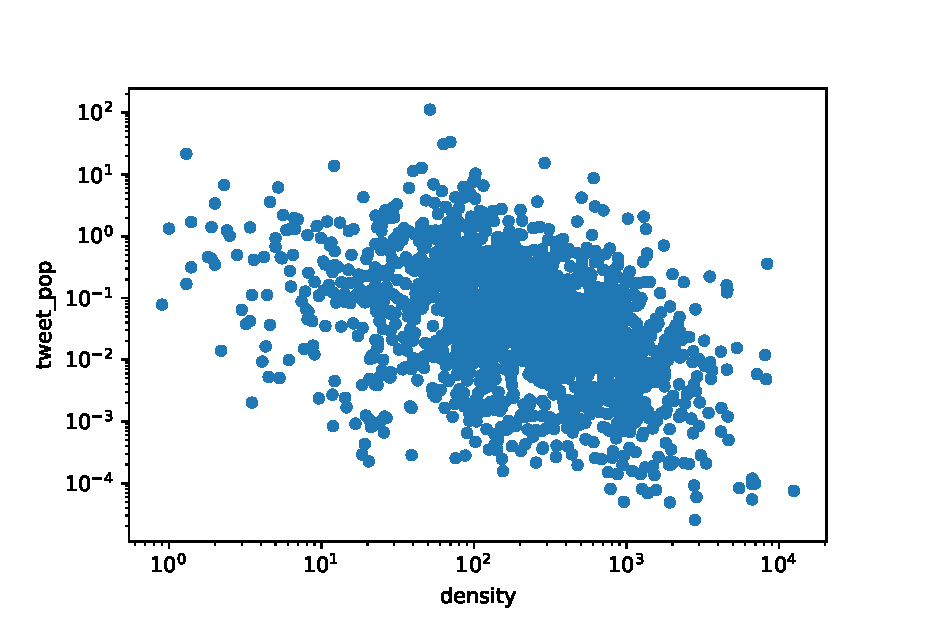
\includegraphics[width=0.5\textwidth]{images/mun_density_pop.eps}
  \caption{We plot the population density vs twitter popularity in each municipality on a log-log scale. The correlation value (of the log values) was -0.398908.}
  \label{mun_pop}
\end{figure}


\begin{figure}[h]
  \includegraphics[width=0.5\textwidth]{images/can_density_pop.eps}
  \caption{We plot the population density vs twitter popularity in each canton on a log-log scale. The correlation value (of the log values) was -0.448168.}
  \label{can_pop}
\end{figure}


%%%%%%%%%%%%%%%%%%%%%%%%%%%%%%%
\subsection{Reconstructing the R\"ostigraben}
To detect the R\"ostigraben, we first exlcuded all English language tweets, then we computed the language which had the highest number of tweets for each municipality. We visualize the results on Figure \ref{rosti_map}. Our results seams very robust and agrees with the official definiton of the R\"ostigraben. This is a very reassuring results given the simplicity of our method and our preliminary concerns with the dataset.

\begin{figure}[h]
  \includegraphics[width=0.5\textwidth]{images/rosti_map.png}
  \caption{The R\"ostigraben reconstructed from the language of the tweets. The color encoding is yellow: French; orange: German, red: Italian}
  \label{rosti_map}
\end{figure}

\begin{figure}[h]
  \includegraphics[width=0.5\textwidth]{images/Map_Languages_CH.png}
  \caption{The R\"ostigraben from its Wikipedia page (originally from admin.ch)}
  \label{rosti_map_wiki}
\end{figure}

\subsection{Political activity}

We have tested four sets of political tweets:
\begin{enumerate}
 \item Tweets collected using only the above initial sets, without any bootstrapping.
\item Tweets collected using bootstrapping using only the above initial sets, without making use of the political user data. The bootstrapping is 3 iterations, with 2 top hashtags that are not present in the existing set added at every iteration.
\item Tweets collected using the above initial sets and the best words extracted (using KL-div) from the political user tweets. We pick the top 15 French hashtags and the top 10 German hashtags.
\item Tweets collected with bootstrapping, using the union of the above sets with words extracted from political user tweets as the initial word set. We perform 3 iterations, picking 2 top hashtags not in the existing word set each time.
\end{enumerate}

In the following figures, the y axis is the ratio of political tweets to all tweets, and the x axis is month and year. Therefore, the plots show the fraction of political tweets in each month. Division by total number of tweets in each month was necessary to account for the imbalances of the dataset.

\begin{figure}[h]
  \includegraphics[width=0.5\textwidth]{images/case1_pol.PNG}
  \caption{Fraction of political tweets per month in case 1: Only hand-made initial set, no bootstrapping}
  \label{case_1_hist}
\end{figure}

\begin{figure}[h]
  \includegraphics[width=0.5\textwidth]{images/case2_pol.PNG}
  \caption{Fraction of political tweets per month in case 2: Bootstrapping with hand-made initial set, without use of the political user set}
  \label{case_2_hist}
\end{figure}

\begin{figure}[h]
  \includegraphics[width=0.5\textwidth]{images/case3_pol.PNG}
  \caption{Fraction of political tweets per month in case 3: Hand-made initial set + set of words extracted from political user tweets, no bootstrap}
  \label{case_3_hist}
\end{figure}

\begin{figure}[h]
  \includegraphics[width=0.5\textwidth]{images/case4_pol.PNG}
  \caption{Fraction of political tweets per month in case 4: Handmade initial set + words extracted from political user tweets + bootstrapping}
  \label{case_4_hist}
\end{figure}

\begin{figure}[h]
  \includegraphics[width=0.5\textwidth]{images/original_users_pol.PNG}
  \caption{Fraction of political tweets per month for the political user tweet set}
  \label{original_user_pol_hist}
\end{figure}

In cases 3 and 4 there are clear spikes around the two federal elections in 2011 and 2015, and also a significant spike at February 2014, which corresponds to a highly controversial referendum regarding migration. The original political user tweets plot shows that our algorithm is clearly superior in terms of detecting political trends, compared to solely using accounts. \\
Looking at the set of hashtags collected using our KL-divergence method (which may be found in our notebook and has been omitted here for the sake of brevity) on the political user tweets, we can see that hashtags such as \#chvote and \#ef2015 (federal elections) appear at the top of the list. In addition, the bootstrapping method adds hashtags such as \#migration to the French word set and \#abst14 (the trending hashtag for the Feb. 2014 referendum) to the German set. Our bootstrapping increases the number of French language tweets from case 3's 15,747 to case 4's 16,595, and the number of German language tweets from case 3's 6,040 to case 4's 8,019. The more significant increase however, comes with the words extracted from the political user tweets, which shows an increase from case 1's 3,522 French and 313 German tweets to 15,747 and 6,040 respectively. 
